\documentclass[11pt]{article}
\usepackage[margin=0.9in]{geometry}
\usepackage[T1]{fontenc}
\usepackage{lmodern,amsmath,amssymb,amsthm,booktabs,longtable,array,graphicx}
\usepackage[hidelinks]{hyperref}
\usepackage{microtype,needspace}
\graphicspath{{../../figures/}{figures/}}
\setlength{\parskip}{4pt}
\setlength{\parindent}{0pt}
\renewcommand{\arraystretch}{1.16}
\newtheorem{proposition}{Proposition}
\newtheorem{theorem}{Theorem}
\newcommand{\R}{\mathbb{R}}
\newcommand{\rank}{\operatorname{rank}}
\newcommand{\tr}{\operatorname{tr}}
\newcommand{\ownership}{\smallskip\textit{Owner: James Cottrell (solo).
Checked by: pending instructor guidance for individual work.}\par\smallskip}
\title{Finding Similar Mandarin Texts\\Using Linear Algebra\\[5pt]
\large Iteration 2: Definitions, Derivations, Data, and Simulation}
\author{James Cottrell\\DS5020 Intro Linear Algebra \& Probability}
\date{November 13, 2026}
\begin{document}
\maketitle
\begin{abstract}
This project represents Mandarin news documents as character-based TF-IDF vectors
and studies similarity before and after truncated singular value decomposition
(SVD). This iteration establishes the mathematics, solves a small example by hand,
describes 300 real news documents, and verifies a from-scratch SVD implementation
on a two-topic simulation. All five assigned math questions are answered. A key
distinction is that projected coordinates $V_k\Sigma_k$ and folded coordinates
$V_k$ use different cosine geometries. The simulation verifies reconstruction and
query identities. Its deliberately separated topics provide a controlled check,
not evidence of general semantic understanding.
\end{abstract}

\section{Scope and individual responsibilities}
The research question is: how does retaining $k$ singular directions change
cosine-based topical similarity among Mandarin texts? Character terms avoid an
additional word-segmentation package. This connects linear algebra to my background
in computer science and linguistics and interest in NLP.

I am the sole student and project leader. The project includes data acquisition,
cleaning, mathematical exposition, implementation, verification, and writing.
The plan distinguishes assisted preparation from student review and checker
sign-off. This iteration explores real data and checks the method on simulation.
Rank selection and the main real-data retrieval evaluation belong to Iteration 3.
SVD is not assumed to improve every similarity comparison.

\section{Notation and formal definitions}
\begin{longtable}{p{.18\textwidth}p{.46\textwidth}p{.27\textwidth}}
\toprule Symbol & Meaning & Dimensions/domain \\ \midrule\endhead
$m,n,r,k$ & Number of terms, documents, rank, retained dimension & $1\le k\le r\le\min(m,n)$ \\
$t,d,i,j$ & Term, document, or singular-direction indices & Valid integer indices \\
$C,A$ & Count and TF-IDF term-document matrices & $\R^{m\times n}$ \\
$C_{td},df_t,w_t$ & Count, document frequency, IDF weight & Nonnegative scalars; $1\le df_t\le n$ for retained terms \\
$U,\Sigma,V$ & Compact SVD factors & $m\times r$, $r\times r$, $n\times r$ \\
$u_i,v_i,\sigma_i$ & Singular vectors and positive singular value & $u_i\in\R^m$, $v_i\in\R^n$, $\sigma_i>0$ \\
$U_k,\Sigma_k,V_k$ & First $k$ singular factors & $m\times k$, $k\times k$, $n\times k$ \\
$A_k,P_k$ & Truncation; projector $U_kU_k^\top$ & $m\times n$; $m\times m$ \\
$D,a_d,d_d$ & Document rows; original and reduced columns & $D=V_k\Sigma_k\in\R^{n\times k}$; $a_d\in\R^m$, $d_d\in\R^k$ \\
$q,z,\widehat q$ & TF-IDF query, projected query, folded query & $q\in\R^m$; $z,\widehat q\in\R^k$ \\
$e_d,I$ & Standard basis vector; identity matrix & $e_d\in\R^n$; $I$ has the required size \\
$B,P,\ell$ & Arbitrary approximation; its column projector; its rank & $B\in\R^{m\times n}$; $P\in\R^{m\times m}$; $\ell\le k$ \\
$G,Q,J$ & Gram matrix, eigenvector matrix, Jacobi rotation & $p\times p$, $p=\min(m,n)$ \\
$T,S$ & Total retained characters; Jacobi sweeps & Nonnegative integers \\
$c,s,t_*,\tau$ & Rotation scalars (not term indices) & Real; $c^2+s^2=1$ \\
$a,b,h$ & Cosine input vectors; query coefficients & $a,b\in\R^m$; $h\in\R^k$ \\
$\lambda_i,b_i$ & Gram eigenvalue; proof weight $\|Pu_i\|_2^2$ & Scalars; $\lambda_i\ge0$; $0\le b_i\le1$ \\
$\alpha$ & Common IDF in the toy example & $\log(3/2)$ \\
$h_d,L,\theta_h$ & Simulated topic, tokens per document, term probabilities & $h_d\in\{0,1\}$; $L=60$; $\theta_h\in[0,1]^{50}$ \\
$p_h,N_h,S_h,\widehat p_h$ & First-half token probability, total tokens, observed count, estimate & Scalars; $N_h=1200$; $\widehat p_h=S_h/N_h$ \\
$X_j,\beta_t,T_q$ & Token indicator, Dirichlet parameter, query length & $X_j\in\{0,1\}$; $\beta_t>0$; $T_q$ integer \\
\bottomrule
\end{longtable}
A vector in $\R^m$ is an ordered list of $m$ real coordinates. Its inner product
with $b$ is $a^\top b=\sum_t a_tb_t$ and its Euclidean norm is
$\|a\|_2=\sqrt{a^\top a}$. Orthogonal vectors have zero inner product.
Orthonormal columns satisfy $U^\top U=I$. The column space
$\mathcal C(A)=\{Ax:x\in\R^n\}$ has dimension $\rank(A)$.
A symmetric matrix $G$ is positive semidefinite when $x^\top Gx\ge0$ for all $x$.
An eigenpair satisfies $Gv=\lambda v$ with $v\ne0$.

The trace $\tr(X)$ is the sum of diagonal entries. The Frobenius inner product is
$\langle X,Y\rangle_F=\tr(X^\top Y)$, and
$\|X\|_F^2=\sum_{t,d}X_{td}^2=\tr(X^\top X)$.
An orthogonal projector onto a subspace satisfies $P=P^\top=P^2$ and has that
subspace as its column space. A rank-$k$ approximation has rank at most $k$.
The compact SVD is $A=U\Sigma V^\top$, where $U^\top U=V^\top V=I_r$ and
$\Sigma=\operatorname{diag}(\sigma_1,\ldots,\sigma_r)$ with
$\sigma_1\ge\cdots\ge\sigma_r>0$.
Other temporary symbols are defined at their first use below.

\clearpage
\section{Assumptions and consequences of failure}
\begin{longtable}{p{.24\textwidth}p{.34\textwidth}p{.33\textwidth}}
\toprule Assumption/choice & If it fails & Planned Iteration 3 check \\ \midrule\endhead
One vocabulary, preprocessing rule, and corpus IDF for documents and queries.
& Dot products would compare different features or scales.
& Freeze vocabulary/IDF; test known and out-of-vocabulary queries. \\
Nonzero original and projected vectors for cosine.
& The cosine denominator would be zero and the angle undefined.
& Count zero vectors and reject unsupported queries explicitly. \\
Positive, numerically resolved retained singular values.
& Inversion is undefined at zero and unstable near zero.
& Report the cutoff and sensitivity to $k$, tolerance, and spectral gaps. \\
Approximately orthonormal computed singular vectors.
& Coordinate cosines need not equal reconstructed-vector cosines.
& Measure $U_k^\top U_k-I$, $V_k^\top V_k-I$, and reconstruction residuals. \\
Topic labels are a useful but imperfect similarity proxy.
& Label agreement may not measure semantic relevance accurately.
& Inspect retrieved examples and distinguish topic from meaning. \\
No selected exact duplicates after preprocessing.
& Duplicate matches could inflate evaluation scores.
& Audit exact duplicates and investigate near-duplicates. \\
The finite prefix sample has limited representativeness.
& Source order could bias results toward particular subtopics or dates.
& Broaden/randomize the candidate pool before corpus-level claims. \\
Independent simulated tokens conditional on chosen topic probabilities.
& Binomial/multinomial variance formulas would change under dependence.
& Check frequencies; do not assume real language satisfies independence. \\
\bottomrule
\end{longtable}
No normality or full-column-rank assumption is needed for the deterministic SVD
identities. Independence is used only in the simulation probability calculation.
The bag-of-characters representation discards word order and compositional meaning.
Simplified/traditional variants are not merged. Raw counts allow document length
to influence the SVD, even though cosine itself is invariant to positive rescaling
of a single vector. No centering is performed; this is latent semantic analysis,
not centered PCA.

\clearpage
\section{Iteration 2 -- Math Questions}
\subsection{Q1: Term-document matrix and TF-IDF}
\ownership
A document is its news title concatenated with its body. A term is a Unicode
character in U+4E00--U+9FFF. Spaces, punctuation, Latin letters, and digits are
removed. The vocabulary is the sorted set of retained characters observed in the
selected corpus. Define
\begin{align}
C_{td}&=\text{number of occurrences of term $t$ in document $d$},\\
df_t&=\sum_{d=1}^{n}\mathbf1\{C_{td}>0\},
&&\text{(document-frequency definition)}\\
\operatorname{TF}_{td}&=C_{td},\qquad w_t=\log(n/df_t),
&&\text{(chosen TF and IDF)}\\
A_{td}&=C_{td}w_t.
&&\text{(TF-IDF definition)}
\end{align}
The indicator $\mathbf1\{E\}$ is one when $E$ holds, zero otherwise. One row of
$A$ represents a character, one column a document, and one entry a character's
corpus-adjusted count. Repetition raises TF, while occurrence across many
documents reduces IDF. A retained corpus term has $df_t>0$; a universal term has
IDF zero. In the simulation, an unobserved fixed-vocabulary term is an all-zero
row and is assigned weight zero without evaluating $\log0$. This produces the
same weighted matrix as the starter's $\log(n/\max(df_t,1))$ convention.
Queries reuse the fitted vocabulary and IDF; they never refit IDF on the query.

\subsection{Q2: Cosine similarity and Cauchy--Schwarz}
\ownership
\begin{proposition}
For nonzero $a,b\in\R^m$, the cosine
$\operatorname{cos}(a,b)=a^\top b/(\|a\|_2\|b\|_2)$ belongs to $[-1,1]$.
\end{proposition}
\begin{proof}
\begin{align*}
|a^\top b|&\le\|a\|_2\|b\|_2 &&\text{(Cauchy--Schwarz)},\\
-\|a\|_2\|b\|_2&\le a^\top b\le\|a\|_2\|b\|_2
&&\text{(definition of absolute value)},\\
-1&\le\frac{a^\top b}{\|a\|_2\|b\|_2}\le1
&&\text{(divide by a positive denominator)}.
\end{align*}
Both norms are positive because both vectors are nonzero. A positive scalar
multiple gives cosine $1$, a negative multiple gives $-1$, and nonzero orthogonal
vectors give $0$, directly by substitution into the definition.
\end{proof}
Original TF-IDF entries are nonnegative, so their defined cosines are in $[0,1]$.
Reduced coordinates can have either sign and require $[-1,1]$. Zero-vector cosine
is undefined; the implementation rejects it rather than reporting zero.

\Needspace{10\baselineskip}
\subsection{Q3: SVD construction, optimality, and tail error}
\ownership
\begin{proposition}[Constructing singular vectors]
$A^\top A$ is symmetric positive semidefinite. For its orthonormal eigenvectors
$v_i$ with positive eigenvalues $\lambda_i$, the definitions
$\sigma_i=\sqrt{\lambda_i}$ and $u_i=Av_i/\sigma_i$ give orthonormal $u_i$.
\end{proposition}
\begin{proof}
\begin{align*}
(A^\top A)^\top&=A^\top A &&\text{(transpose rule)},\\
x^\top A^\top Ax&=(Ax)^\top(Ax)=\|Ax\|_2^2\ge0
&&\text{(associativity and norm definition)}.
\end{align*}
The real symmetric spectral theorem supplies real eigenvalues and an orthonormal
eigenbasis. A unit eigenvector gives
$\lambda_i=v_i^\top A^\top Av_i=\|Av_i\|_2^2\ge0$ by the eigenvector equation.
For positive eigenvalues,
\begin{align*}
u_i^\top u_j
&=\frac{v_i^\top A^\top Av_j}{\sigma_i\sigma_j}
&&\text{(substitute definitions)}\\
&=\frac{\lambda_jv_i^\top v_j}{\sigma_i\sigma_j}
&&\text{(eigenvector equation)}\\
&=\begin{cases}1&i=j,\\0&i\ne j,\end{cases}
&&\text{(orthonormality and $\lambda_i=\sigma_i^2$)}.
\end{align*}
For a zero eigenvalue, $\|Av\|_2^2=0$ implies $Av=0$. Expanding any input
in the complete right eigenbasis therefore gives
$A=\sum_{i=1}^r\sigma_i u_iv_i^\top=U\Sigma V^\top$.
\end{proof}

The standard approximation theorem is stated in \cite{ey}; the following proof
uses an orthogonal-projector argument and explicitly derives the error bound.
\begin{theorem}[Eckart--Young, Frobenius form]
For $A=U\Sigma V^\top$ of rank $r$ and $1\le k\le r$, define
$A_k=\sum_{i=1}^k\sigma_i u_iv_i^\top=U_k\Sigma_kV_k^\top$. Then
\[
\min_{\rank(B)\le k}\|A-B\|_F^2
=\|A-A_k\|_F^2=\sum_{i=k+1}^{r}\sigma_i^2.
\]
\end{theorem}
\begin{proof}
First, the rank-one matrices are orthonormal in Frobenius inner product:
\[
\langle u_iv_i^\top,u_jv_j^\top\rangle_F
=\tr(v_iu_i^\top u_jv_j^\top)
=(u_i^\top u_j)(v_j^\top v_i)=\mathbf1\{i=j\}
\]
by the trace rule and orthonormality. Thus
\[
\|A-A_k\|_F^2
=\left\|\sum_{i=k+1}^{r}\sigma_i u_iv_i^\top\right\|_F^2
=\sum_{i=k+1}^{r}\sigma_i^2
\]
by Pythagoras in the Frobenius inner product.

To prove optimality among all rank-at-most-$k$ matrices, let $P$ project onto
$\mathcal C(B)$, whose dimension is $\ell\le k$. Because $P(I-P)=0$,
$(I-P)A$ and $PA-B$ are orthogonal in Frobenius inner product. Therefore
\begin{align*}
\|A-B\|_F^2&=\|(I-P)A\|_F^2+\|PA-B\|_F^2
&&\text{(orthogonal decomposition)}\\
&\ge\|A\|_F^2-\|PA\|_F^2
&&\text{(nonnegativity and Pythagoras)}.
\end{align*}
Let $b_i=\|Pu_i\|_2^2$. Projection cannot increase length, so $0\le b_i\le1$.
Complete the left singular vectors to an orthonormal basis; the sum of all
projected squared basis lengths is $\tr(P)=\ell$. In particular,
$\sum_{i=1}^r b_i\le\ell\le k$. Also
\[
\|PA\|_F^2=\tr(PAA^\top)=\sum_{i=1}^r\sigma_i^2b_i
\]
by $P=P^\top=P^2$, the cyclic trace rule, and the SVD. Since the singular values
decrease,
\begin{align*}
\sum_{i=1}^r\sigma_i^2b_i
&\le\sum_{i=1}^k\sigma_i^2b_i+\sigma_k^2\sum_{i>k}b_i
&&\text{(ordered singular values)}\\
&\le\sum_{i=1}^k\bigl[\sigma_i^2b_i+\sigma_k^2(1-b_i)\bigr]
&&\text{($\sum_i b_i\le k$)}\\
&\le\sum_{i=1}^k\sigma_i^2
&&\text{($b_i\le1$ and $\sigma_k^2\le\sigma_i^2$)}.
\end{align*}
Thus $\|A-B\|_F^2\ge\sum_{i>k}\sigma_i^2$, and $A_k$ attains the bound.
Its rank is $k$ since all retained singular values are positive.
\end{proof}
Optimal reconstruction in this norm does not imply optimal topic retrieval.
Ties at the truncation boundary can make the best approximation nonunique.
The same orthonormal expansion gives $\|A\|_F^2=\sum_i\sigma_i^2$, so the
retained energy fraction is $\sum_{i\le k}\sigma_i^2/\sum_i\sigma_i^2$ when $A\ne0$.

\subsection{Q4: Reduced document coordinates}
\ownership
\begin{proposition}
The projected coordinates of $a_d=Ae_d$ are
$d_d=U_k^\top a_d=\Sigma_kV_k^\top e_d$. Row $d$ of $D=V_k\Sigma_k$ is
$d_d^\top$. Cosines between nonzero reconstructed columns of $A_k$ equal cosines
between the corresponding rows of $D$.
\end{proposition}
\begin{proof}
\begin{align*}
U_k^\top A&=U_k^\top U\Sigma V^\top &&\text{(substitute SVD)}\\
&=\Sigma_kV_k^\top &&\text{(orthonormal columns select the first $k$ rows)}.
\end{align*}
Multiply by $e_d$ to select document $d$ and transpose to identify its row of $D$.
Its reconstruction is $A_ke_d=U_kd_d$ by the definition of $A_k$. For nonzero
projected documents,
\begin{align*}
(U_kd_i)^\top(U_kd_j)&=d_i^\top d_j &&\text{($U_k^\top U_k=I$)},\\
\|U_kd_i\|_2^2&=d_i^\top d_i=\|d_i\|_2^2 &&\text{(same identity)}.
\end{align*}
Substitute both equalities into the cosine definition to prove the result.
\end{proof}
Original columns $a_d$ generally differ from $A_ke_d$. Q4 preserves angles
between reconstructed columns and their coordinates, not between all original
and reconstructed document pairs.

\subsection{Q5: Mapping a new query}
\ownership
\begin{proposition}
For positive retained singular values, the unique $h\in\R^k$ minimizing
$\|q-U_k\Sigma_kh\|_2^2$ is $\widehat q=\Sigma_k^{-1}U_k^\top q$.
\end{proposition}
\begin{proof}
Set $P_k=U_kU_k^\top$. Transposition gives $P_k=P_k^\top$, and
$P_k^2=U_k(U_k^\top U_k)U_k^\top=P_k$, so it is the orthogonal projector onto
$\mathcal C(U_k)$. Adding and subtracting $P_kq$ gives
\[
q-U_k\Sigma_kh=(I-P_k)q+U_k(U_k^\top q-\Sigma_kh).
\]
The terms are orthogonal, and Q4 shows that $U_k$ preserves the norm of a
$k$-vector. Hence, by Pythagoras,
\[
\|q-U_k\Sigma_kh\|_2^2
=\|(I-P_k)q\|_2^2+\|U_k^\top q-\Sigma_kh\|_2^2.
\]
The first term is independent of $h$; the second is nonnegative and is zero when
$\Sigma_kh=U_k^\top q$. The positive diagonal makes $\Sigma_k$ invertible,
giving the unique solution $h=\Sigma_k^{-1}U_k^\top q$.
\end{proof}
For an existing document $q=Ae_d$, Q4 gives
$\widehat q=\Sigma_k^{-1}\Sigma_kV_k^\top e_d=V_k^\top e_d$.
This is its row of $V_k$, transposed, exactly as the assigned starter checks.

For Q4's retrieval geometry compare $z=U_k^\top q=\Sigma_k\widehat q$ with rows
of $D=V_k\Sigma_k$. Alternatively compare $\widehat q$ with rows of $V_k$ if
folded geometry is deliberately desired. Unequal axis rescaling changes angles;
these two comparisons need not agree. A component of $q$ outside the retained
subspace remains in the residual and is not reconstructed by folding.

\section{Small example solved completely by hand}
Use two toy character terms and three documents: two copies of term 1; two copies
of term 2; and one copy of each. Thus
\[
C=\begin{bmatrix}2&0&1\\0&2&1\end{bmatrix},\quad df_1=df_2=2,
\quad\alpha=\log(3/2),\quad A=\alpha C.
\]
The smaller Gram matrix is
$AA^\top=\alpha^2\begin{bmatrix}5&1\\1&5\end{bmatrix}$.
The characteristic polynomial factors as
\[
\det(AA^\top-\lambda I)=(5\alpha^2-\lambda)^2-\alpha^4
=(\lambda-6\alpha^2)(\lambda-4\alpha^2).
\]
The eigenvalues are $6\alpha^2$ and $4\alpha^2$. For the first eigenvalue,
the null-system equation is $-u_1+u_2=0$, so the coordinates are equal.
For the second, $u_1+u_2=0$, so they are opposite. Normalizing these two
directions gives
\[
U=\frac1{\sqrt2}\begin{bmatrix}1&1\\1&-1\end{bmatrix},\qquad
\Sigma=\alpha\begin{bmatrix}\sqrt6&0\\0&2\end{bmatrix}.
\]
The rule $v_i=A^\top u_i/\sigma_i$ then yields
\[
V=\begin{bmatrix}1/\sqrt3&1/\sqrt2\\1/\sqrt3&-1/\sqrt2\\1/\sqrt3&0\end{bmatrix}.
\]
Its columns have unit length and zero dot product by direct substitution.
Multiplication verifies $U\Sigma V^\top=A$. Retaining one direction gives
\[
A_1=\alpha\begin{bmatrix}1&1&1\\1&1&1\end{bmatrix},\qquad
A-A_1=\alpha\begin{bmatrix}1&-1&0\\-1&1&0\end{bmatrix}.
\]
The four squared nonzero errors sum to $4\alpha^2=\sigma_2^2$, checking Q3.
Total energy is $10\alpha^2$ and retained energy is $6\alpha^2$, or $60\%$.
The original cosine of documents 1 and 2 is zero. Documents 1 and 3 have cosine
$2\alpha^2/(2\alpha\sqrt2\alpha)=1/\sqrt2$. Rank one makes all projected
coordinates the positive scalar $\sqrt2\alpha$, so every cosine becomes $1$.
Over-reduction has erased the distinction between originally orthogonal documents.

For query $q=a_1=(2\alpha,0)^\top$,
$z=(\sqrt2\alpha,\sqrt2\alpha)^\top$ and
$\widehat q=(1/\sqrt3,1/\sqrt2)^\top$, agreeing with the corresponding rows
of $D$ and $V$. Folded cosine for documents 1 and 2 is
$(1/3-1/2)/(1/3+1/2)=-1/5$; for documents 1 and 3 it is $\sqrt{2/5}$.
This explicitly demonstrates the query-coordinate scaling distinction.
\par
\begin{table}[htbp]\centering
\small
\caption{Independent hand-example checks.}
\begin{tabular}{lrr}\toprule
Quantity & Hand value & Code value \\ \midrule
Original cosine, documents 1 and 2 & $0$ & 0.000000 \\
Original cosine, documents 1 and 3 & $1/\sqrt2$ & 0.707107 \\
Folded cosine, documents 1 and 2 & $-1/5$ & -0.200000 \\
Folded cosine, documents 1 and 3 & $\sqrt{2/5}$ & 0.632456 \\
Squared rank-one error & $4\log^2(3/2)$ & 0.657608 \\
\bottomrule\end{tabular}
\end{table}
\par

The script \texttt{src/verify.py} reproduces the hand calculations:
$\sigma_1=0.993183$, $\sigma_2=0.810930$, and rank-one squared error $0.657608$.

\section{Algorithm as mathematics, dimensions, and costs}
The core numerical routine implements cyclic Jacobi rotations on the smaller
Gram matrix; no library eigensolver or SVD solver generates its output.
The following are dense upper bounds, with $p=\min(m,n)$ and $S$ Jacobi sweeps.
\begin{enumerate}
\item Scan $T$ retained characters, sort the vocabulary, and form
$C\in\R^{m\times n}$. Cost $O(T+m\log m+mn)$ including dense allocation;
storage $O(mn)$.
\item Compute $df,w\in\R^m$ and $A_{td}=C_{td}w_t$.
Cost $O(mn)$ arithmetic/comparisons and $m$ logarithms; $A$ is $m\times n$.
\item Form $G=A^\top A$ for $n\le m$, otherwise $G=AA^\top$.
$G$ is $p\times p$; cost $O(mnp)$, extra storage $O(p^2)$.
\item Set $Q=I_p$ and visit each off-diagonal pair $a<b$ cyclically. For
non-negligible $g_{ab}$, define
\[
\tau=\frac{g_{bb}-g_{aa}}{2g_{ab}},\quad
t_*=\frac{\operatorname{sgn}_+(\tau)}{|\tau|+\sqrt{1+\tau^2}},\quad
c=\frac1{\sqrt{1+t_*^2}},\quad s=t_*c,
\]
where $\operatorname{sgn}_+(0)=1$. Set $J$ to identity except for its $(a,b)$
block $\begin{bmatrix}c&s\\-s&c\end{bmatrix}$. Update
$G\leftarrow J^\top GJ$, $Q\leftarrow QJ$ using affected rows/columns only.
Orthogonal similarity preserves eigenvalues, and the chosen rotation annihilates
the selected off-diagonal entry. Each rotation costs $O(p)$, so $S$ sweeps cost
$O(Sp^3)$. Stop when the off-diagonal Frobenius norm is at most $10^{-12}$ times
the initial Gram norm; fail explicitly if 100 sweeps do not reach this tolerance.
\item Sort eigenvalues descending; retain $\lambda_i>10^{-12}\lambda_{\max}$.
Set $\sigma_i=\sqrt{\lambda_i}$ and compute the other vectors via
$u_i=Av_i/\sigma_i$ or $v_i=A^\top u_i/\sigma_i$.
Factor sizes are $m\times r$, $r\times r$, $n\times r$.
Cost $O(p\log p+mnr)$. The cutoff excludes unresolved near-zero modes.
\item Choose $k\le r$, form $D=V_k\Sigma_k\in\R^{n\times k}$, and normalize
nonzero rows: $O(nk)$. Multiplying the normalized matrix by its transpose gives
all cosines in $O(n^2k)$ and uses $O(n^2)$ output storage.
\item Build $q\in\R^m$ using corpus vocabulary/IDF; form $z=U_k^\top q\in\R^k$.
For $T_q$ query characters, construction, projection, and all document scores cost
$O(T_q+m+mk+nk)$. Folded coordinates add $k$ divisions by singular values if used.
\end{enumerate}
The nonzero condition number is $\sigma_1/\sigma_r$; the ratio of positive Gram
eigenvalues is its square because $\lambda_i=\sigma_i^2$.
This Gram approach may therefore lose relative
accuracy in very small singular values. It is an educational algorithm for the
small verified matrices here, not a production-scale SVD claim. Convergence,
orthogonality, cutoff, and library agreement are checked explicitly. The
\texttt{numpy.linalg.svd} calls occur only after the custom decomposition in
verification scripts. This follows the stricter general project policy despite
the handout's direct library-SVD starter.

\section{Real dataset and exploratory description}
\subsection{Source and sampling}
The original THUNLP source describes THUCNews as Chinese news from Sina RSS
channels \cite{thuctc}. For a practical download this project uses the Tongjilibo
JSONL mirror \cite{mirror}, pinned to revision
\texttt{ae77e363396e90b54cdaa9eafdbc5e102a3d4019}, accessed November 13, 2026.
The mirror labels the dataset Apache-2.0. Article texts remain local; the
repository distributes acquisition code and sample IDs rather than the raw news.

Download the first 1,000 records each from sports, education, and technology.
Concatenate title and body, retain at least 30 Chinese characters, and remove
exact duplicates after filtering. Sample 100 eligible documents per category
without replacement using \texttt{np.random.default\_rng(0)} in that category order.
Sort the sampled source rows for stable output. This is a random sample of a
finite eligible prefix, not of all THUCNews; source ordering can bias subtopics
and dates. Source URLs, revision, prefix SHA-256 hashes, and chosen row IDs are
recorded for reproduction.

\subsection{Variables, missingness, and matrix shape}
The source fields are \texttt{id}, \texttt{title}, and \texttt{content}, all
strings. Each field has zero missing values across the 3,000 examined source
records. The processed document table has 300 rows and four columns:
\texttt{document\_id} (string), \texttt{category} (string), \texttt{text} (string),
and \texttt{character\_count} (integer), with no missing values. These document
rows differ from the mathematical matrix orientation: $A$ has 3,123 character
rows and 300 document columns. It has 94,011 nonzero entries, density $10.0343\%$.
No selected document is duplicated after filtering, no TF-IDF column is zero,
and this sample has no universal zero-IDF term.
\begin{table}[htbp]\centering
\caption{Observed real-data sample, using retained Chinese character lengths.}
\begin{tabular}{lr}\toprule Quantity & Value \\ \midrule
Documents per category & 100 \\
Total documents & 300 \\
Vocabulary terms & 3,123 \\
Minimum / median / maximum length & 72 / 788 / 3,962 \\
Mean length & 928.34 \\
Zero TF-IDF documents & 0 \\
\bottomrule\end{tabular}\end{table}
\begin{figure}[htbp]\centering
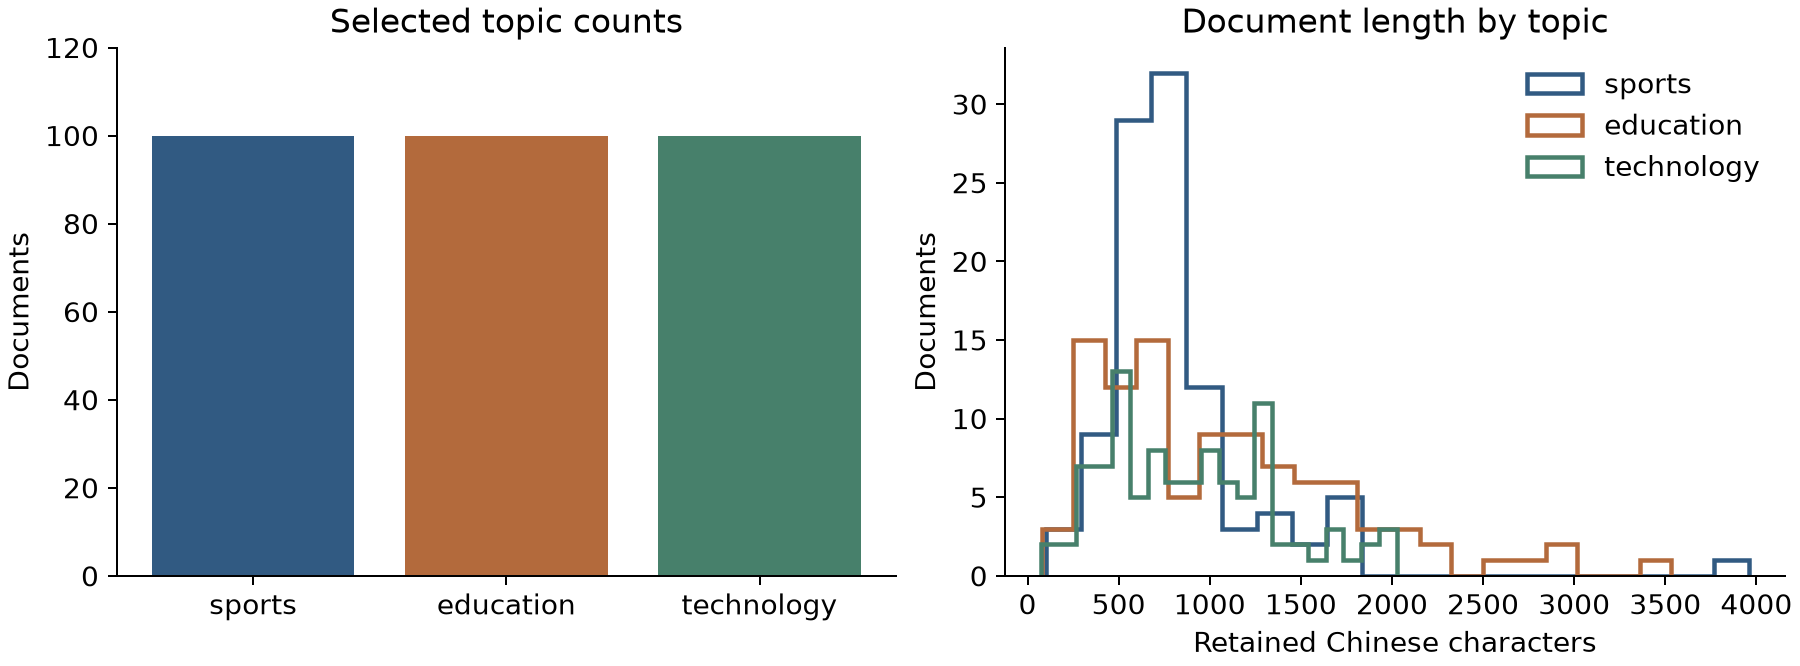
\includegraphics[width=\textwidth]{data_overview.png}
\caption{Two exploratory plots: topic counts and retained-character length
distributions. Equal counts are imposed by sampling. Document sizes vary
substantially, motivating attention to weighting in the later experiment.}
\end{figure}
Only data description and matrix construction are performed on this corpus in
Iteration 2. Topic labels are excluded from counts, weighting, and the mathematical
method. No real-data retrieval performance is claimed yet.

\section{Simulation Check}
\subsection{Model and known truth}
Use seed 0, 50 terms, 40 documents, and 20 documents per hidden topic. Draw topic
probability vectors once from
\begin{align*}
\theta_0&\sim\operatorname{Dirichlet}(\underbrace{2,\ldots,2}_{25},
\underbrace{0.1,\ldots,0.1}_{25}),\\
\theta_1&\sim\operatorname{Dirichlet}(\underbrace{0.1,\ldots,0.1}_{25},
\underbrace{2,\ldots,2}_{25}).
\end{align*}
The Dirichlet distribution is a probability distribution on the simplex
$\{\theta_t\ge0:\sum_t\theta_t=1\}$, with density proportional to
$\prod_t\theta_t^{\beta_t-1}$ for positive parameters $\beta_t$.
Conditional on these realized probability vectors, generate each count column as
\[
C_{:d}\mid h_d,\theta_{h_d}\sim\operatorname{Multinomial}(60,\theta_{h_d}).
\]
This multinomial counts outcomes of 60 independent categorical token draws with
the chosen term probabilities. Topic 0 mainly favors the first 25 terms; topic 1
mainly favors the remaining 25. Apply Q1 weighting and the custom SVD with $k=2$.
Known truth consists of topic labels and chosen probabilities. The realized
sample matrix is not exactly rank two: its computed numerical rank is 40.

\subsection{Probability and variance calculation}
Fix a realized topic distribution and let $p_h=\sum_{t=1}^{25}\theta_{h,t}$.
Let $X_j$ indicate whether token $j$ belongs to the first 25 terms. Then
$E[X_j\mid\theta_h]=p_h$ by the indicator definition, and
$\operatorname{Var}(X_j\mid\theta_h)=p_h(1-p_h)$ since $X_j^2=X_j$.
With $N_h=20\cdot60=1200$, $S_h=\sum_{j=1}^{N_h}X_j$, and
$\widehat p_h=S_h/N_h$,
\begin{align*}
E[S_h\mid\theta_h]&=N_hp_h &&\text{(linearity of expectation)},\\
E[\widehat p_h\mid\theta_h]&=p_h &&\text{(scale by $1/N_h$)},\\
\operatorname{Var}(\widehat p_h\mid\theta_h)&=\frac{p_h(1-p_h)}{N_h}
&&\text{(independent variances add and scale)}.
\end{align*}
Thus the frequency estimate is unbiased, with theoretical standard error equal
to the square root of that variance. Independence is used in the variance step.
\par
\begin{table}[htbp]\centering
\small
\caption{Known and estimated first-half token probabilities.}
\begin{tabular}{rrrrrr}\toprule
Topic & Tokens & Observed count & True $p_h$ & Estimate & True SE \\ \midrule
0 & 1200 & 1127 & 0.939402 & 0.939167 & 0.006888 \\
1 & 1200 & 61 & 0.057946 & 0.050833 & 0.006745 \\
\bottomrule\end{tabular}
\end{table}
\par

Topic 0's first-half probability is about $94\%$, while topic 1's is about $6\%$.
The estimates fluctuate because tokens are sampled. These standard errors describe
the synthetic token model; they do not quantify real-news retrieval uncertainty.

\subsection{Numerical identities}
\par
\begin{table}[htbp]\centering
\small
\caption{Measured numerical agreement (seed 0).}
\begin{tabular}{lr}\toprule
Check & Measured error \\ \midrule
Projected document identity, max absolute error & $5.60\times10^{-13}$ \\
Projected query versus row of $D$ & $3.10\times10^{-13}$ \\
Folded query versus row of $V_k$ & $6.88\times10^{-15}$ \\
Reconstructed versus coordinate cosines & $1.22\times10^{-15}$ \\
Custom versus library singular values & $2.13\times10^{-14}$ \\
Custom versus library rank-two reconstruction & $3.07\times10^{-13}$ \\
\bottomrule\end{tabular}
\end{table}
\par

The solver used eight Jacobi sweeps, reaching relative off-diagonal Gram norm
$1.82\times10^{-13}$. Maximum $U$ and $V$ orthogonality errors were
$4.12\times10^{-11}$ and $9.55\times10^{-15}$, respectively. Full reconstruction
error was $7.02\times10^{-14}$ per entry at worst. Matrix squared Frobenius energy
and summed squared singular values both equal approximately $5249.240$.
\par
\begin{table}[htbp]\centering
\small
\caption{Squared reconstruction error and discarded singular-value energy.}
\begin{tabular}{rrrr}\toprule
$k$ & Measured error & Tail energy & Absolute difference \\ \midrule
1 & 3223.223442 & 3223.223442 & $1.36\times10^{-12}$ \\
2 & 1346.756029 & 1346.756029 & 0.000000 \\
5 & 987.390585 & 987.390585 & $5.68\times10^{-13}$ \\
10 & 619.690285 & 619.690285 & $6.82\times10^{-13}$ \\
40 & $3.52\times10^{-25}$ & 0.000000 & $3.52\times10^{-25}$ \\
\bottomrule\end{tabular}
\end{table}
\par

The tail-energy identity is checked at multiple ranks; the full-rank residual is
roundoff. The custom singular values agree with the library result to
$2.13\times10^{-14}$. The library is used only as a final check.

\subsection{Similarity and interpretation}
\par
\begin{table}[htbp]\centering
\small
\caption{Synthetic topic similarity, excluding self-pairs.}
\begin{tabular}{lrrr}\toprule
Representation & Within topic & Across topics & Same-topic NN rate \\ \midrule
Original TF-IDF & 0.729660 & 0.018342 & 1.000000 \\
Rank-2 SVD & 0.999877 & 0.024643 & 1.000000 \\
\bottomrule\end{tabular}
\end{table}
\par

Within-topic averages exclude self-pairs. Both statistics average ordered pairs;
symmetry makes this equal to the unordered-pair mean. Nearest-neighbor rates
exclude the query itself and use the first index deterministically if scores tie.
\begin{figure}[htbp]\centering
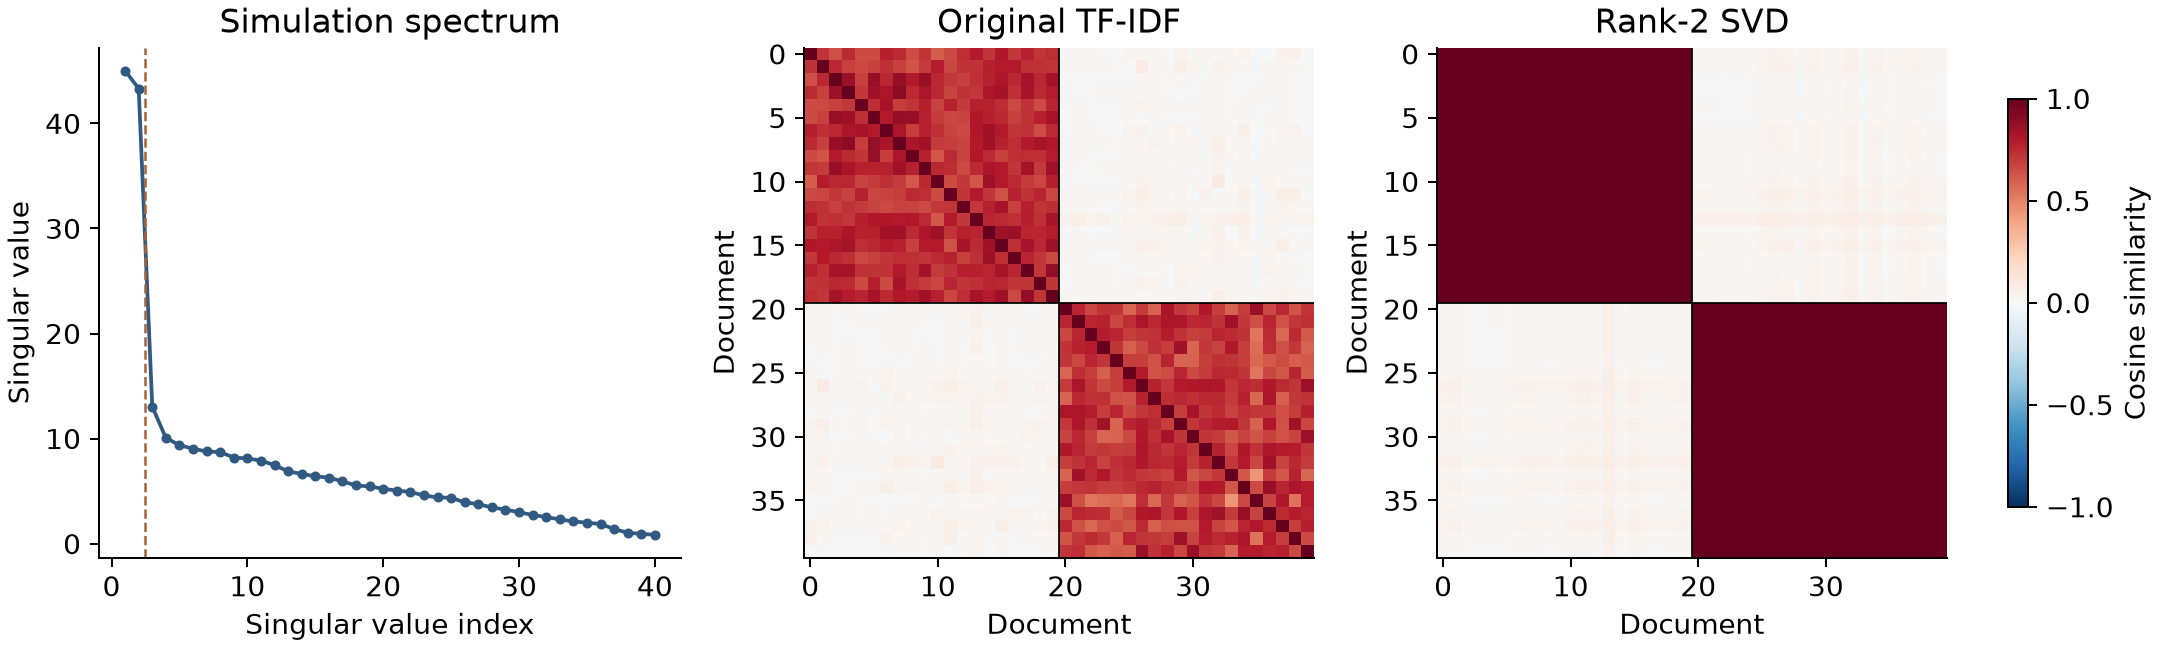
\includegraphics[width=\textwidth]{simulation_overview.png}
\caption{Seed-0 simulation spectrum and cosine matrices. Documents 0--19 have
topic 0; 20--39 have topic 1. Two leading directions emphasize the deliberately
planted structure. Each plotted matrix includes its diagonal for display only.}
\end{figure}
Rank two raises within-topic cosine from $0.729660$ to $0.999877$, but across-topic
cosine also rises slightly, from $0.018342$ to $0.024643$. Both representations
already have same-topic nearest neighbors for all 40 documents. This demonstrates
more concentrated planted geometry, not improved nearest-neighbor accuracy.
Reduced cosines range from $-0.006668$ to $1$ within numerical tolerance.

\Needspace{6\baselineskip}
Each derivation has a corresponding check:
\begin{enumerate}
\item Q1: every simulated column contains 60 tokens; explicit frequency weighting
is used; universal and absent-term cases are checked separately.
\item Q2: nonzero-vector cosines obey the bounds; zero-vector requests are rejected.
\item Q3: reconstruction and the discarded-energy table agree; the independent
hand example checks rank-one error directly.
\item Q4: $U_k^\top A=\Sigma_kV_k^\top$ agrees to $5.60\times10^{-13}$, and
coordinate/reconstructed cosines agree to $1.22\times10^{-15}$.
\item Q5: the existing-document query returns its folded row to
$6.88\times10^{-15}$ and its projected row to $3.10\times10^{-13}$.
\end{enumerate}
These are implementation checks, not substitutes for proofs. Tall, wide,
rank-deficient, repeated-singular-value, and zero matrices also pass comparison
with a library reference; the worst reconstruction error there is
$3.11\times10^{-15}$. Signs and bases within repeated singular subspaces need
not match entrywise, so reconstructions and singular values are compared instead.

\section{Reproducibility and next iteration}
The README gives the commands to acquire data, verify, simulate, describe data,
and rebuild this report. Source hashes, selected IDs, measured CSVs, and figures
are preserved. The environment uses Python 3.12, NumPy 2.5.4, pandas 3.1.1,
Matplotlib 3.11.2, and SciPy 1.18.1; versions are pinned in the requirements files.
NumPy supplies basic array operations; pandas handles tables and Matplotlib plots.
Standard-library imports handle files, network acquisition, and report building.
No additional numerical/NLP package or core library decomposition is used.

Iteration 3 will compare original and reduced real-data representations across
predeclared ranks, inspect retrieval examples, and check near-duplicates and
sampling limitations. Held-out queries must reuse training vocabulary/IDF, and
rank selection must not use final test labels. The toy counterexample warns
against excessive reduction; the simulation establishes a verified baseline.

\appendix
\section{Mathematical appendix and ownership record}
Sections 2, 4, and 5 contain the definitions, full derivations, and hand example to
carry into the final report's math appendix. They are retained in one location
rather than duplicated. The Excel plan records the sole student owner and
assisted preparation separately. Independent checker/signature guidance has not
been supplied, so no independent check or signature is claimed. The author must
review the work and be able to explain each derivation at check-in. The report,
code, and calculations were prepared with AI assistance.

\begin{thebibliography}{9}
\bibitem{assignment} DS5020, \emph{Final Project -- Iteration 2: The Math Foundation},
Fall 2026, pp. 1--3 and 15--16. Supplied course handout; the November 13 copy is identical.
\bibitem{ideas} DS5020, \emph{Final Project Ideas}, Fall 2026, pp. 1--2.
\bibitem{thuctc} THUNLP, \emph{THUCTC: An Efficient Chinese Text Classifier},
THUCNews dataset description. \url{https://github.com/thunlp/THUCTC}.
Accessed November 13, 2026.
\bibitem{mirror} Tongjilibo, \emph{THUCNews JSONL mirror}.
\url{https://huggingface.co/datasets/Tongjilibo/THUCNews}.
Revision and hashes are recorded in \texttt{data/source\_manifest.json}.
Accessed November 13, 2026.
\bibitem{ey} David Bindel, \emph{Matrix nearness problems}, CS 6210,
Cornell University, October 15, 2025. Low-rank approximation theorem reference.
\url{https://www.cs.cornell.edu/courses/cs6210/2025fa/lec/2025-10-15.html}.
The proof here uses an orthogonal-projector argument.
\end{thebibliography}
\end{document}
